\begin{figure}[htbp]\centering
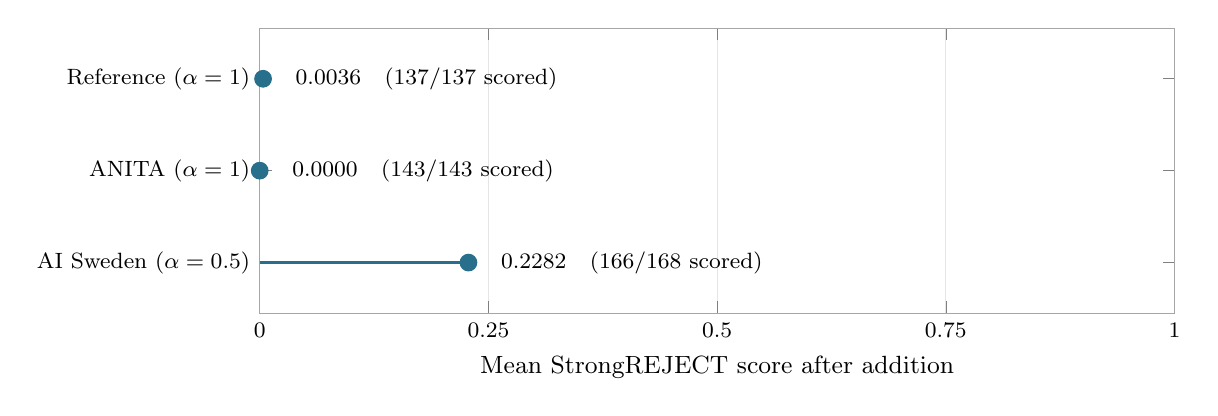
\begin{tikzpicture}
\definecolor{mechblue}{HTML}{286F8C}\definecolor{mechorange}{HTML}{A64B39}
\begin{axis}[width=13.2cm,height=5.2cm,xmin=0,xmax=1,ymin=-.55,ymax=2.55,ytick={0,1,2},yticklabels={AI Sweden ($\alpha=0.5$),ANITA ($\alpha=1$),Reference ($\alpha=1$)},xlabel={Mean StrongREJECT score after addition},xtick={0,.25,.5,.75,1},tick label style={font=\footnotesize},label style={font=\small},axis line style={black!35},xmajorgrids,grid style={black!10},clip=false]
\addplot[mechblue,thick,forget plot] coordinates {(0,2)(0.003649635036,2)};
\addplot[only marks,mark=*,mark size=3pt,mechblue,forget plot] coordinates {(0.003649635036,2)};
\node[anchor=west,font=\footnotesize] at (axis cs:0.028649635036,2) {0.0036\quad(137/137 scored)};
\addplot[mechblue,thick,forget plot] coordinates {(0,1)(0.000000000000,1)};
\addplot[only marks,mark=*,mark size=3pt,mechblue,forget plot] coordinates {(0.000000000000,1)};
\node[anchor=west,font=\footnotesize] at (axis cs:0.025000000000,1) {0.0000\quad(143/143 scored)};
\addplot[mechblue,thick,forget plot] coordinates {(0,0)(0.228162650602,0)};
\addplot[only marks,mark=*,mark size=3pt,mechblue,forget plot] coordinates {(0.228162650602,0)};
\node[anchor=west,font=\footnotesize] at (axis cs:0.253162650602,0) {0.2282\quad(166/168 scored)};
\end{axis}
\end{tikzpicture}
\caption[Graded scores after refusal-direction addition]{Mean graded scores after addition at the reported, post-hoc strengths. The denominator shown beside each point is scored responses out of generated responses; two AI Sweden responses are unscored. These are reused, outcome-selected prompts at different strengths, with no zero-strength rerun or independent controls. A low score can also reflect irrelevant or degenerate output; it is not by itself evidence of successful refusal.}\label{fig:mechanistic-intervention-scores}
\fonte{Author.}
\end{figure}
